
\section{Greedy Search}
\begin{frame}{}{}
  \begin{center}
    {\bf Part VI: Greedy Search}
  \end{center}
\end{frame}

%%%% 3.4 Greedy
\begin{frame}
  \frametitle{The Greedy Search Algorithm}

  Definition: The Greedy Algorithm makes a {\bf locally optimal choice} at each step.
  \bigskip

  Common implementation:
  \begin{itemize}
    \item The solution in broken in "steps";
    \item Sort the input, so the "best step" is first;
    \item Remove the first step from the input, add to the output;
    \item Repeat.
  \end{itemize}

  \begin{block}{Be Careful}
    \begin{itemize}
      \item If the "best step" is wrong, you will get {\bf wrong answer};
      \item Some problems CANNOT be solved by greedy method;
      \item Calculate your "best step" carefully on paper; {\bf Check for trick cases}.
    \end{itemize}
  \end{block}

\end{frame}

\subsection{Example 1}
\begin{frame}{Example Greedy: ICPC Team Selection}
  \begin{block}{}
    \begin{itemize}
      \item You have $3*n$ students to separate in $n$ teams of $3$ students.
      \item Each student has a skill between 1 and 100. Each team has score = median score.
      \item Choose teams to maximize total score.
    \end{itemize}
  \end{block}
  \begin{itemize}
    \item {\bf Example}: Student scores $\{4, 8, 6, 8, 10, 9\}$
    \item Team selection example 1: $\{6, 8, 10\}, \{4, 8, 9\}$: Total 16
    \item Team selection example 2: $\{6, 9, 10\}, \{4, 8, 8\}$: Total 17
  \end{itemize}
\end{frame}

\begin{frame}{Example Greedy: ICPC Team Selection}
  Greedy Algorithm:
  \begin{itemize}
    \item Separate problem into steps;
    \item Select the best step from the input;
    \item Repeat
  \end{itemize}\bigskip

  For this problem, one step is "select a team fron the input".\bigskip

  We can think of many ways to select the "best" team. Which one is correct?
  \begin{itemize}
    \item Select the best 3 students
    \item Select 2 best, 1 worst student
    \item Select 1 best, 2 worst student
    \item Select Best, median, worst student
    \item Other?
  \end{itemize}\bigskip

  Test it on pen and paper!
\end{frame}


\subsection{Example 2}
\begin{frame}
  \frametitle{Traditional Greedy Search: Minimal Coverage}

  \begin{block}{}
    \begin{itemize}
      \item {\bf Input}: integers $A, B$, and a set of $n$ intervals $S =
          [(a_1,b_1), (a_2,b_2), \ldots (a_n,b_n)]$.
      \item {\bf Output} Minimal subset of $S$ that completely covers $A,B$.
    \end{itemize}
  \end{block}

  \bigskip

  \begin{itemize}
  \item A = 10, B = 50;\bigskip


  \item S = [(5, 15), (8, 12), (40, 60), (30, 40), (20, 40), (13, 25),
    (33, 55), (18, 30)]
  \end{itemize}

  \[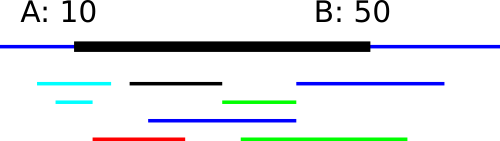
\includegraphics[width=0.6\textwidth]{img/minimal_coverage}\]
\end{frame}

\begin{frame}{Traditional Greedy Search: Minimal Coverage}

  \begin{itemize}
    \item Greedy Step: Choose an interval that covers position $C$
    \item Initial Step: $C = A$
    \item "Best" Step:
    \begin{itemize}
      \item Sort $S$ by left value; Select subset $S_c$ where $C \in s_i$
      \item Choose $s_i$ with largest right value.
    \end{itemize}
    \item $C$ becomes the right value of the interval;
  \end{itemize}
  \vfill

  \begin{block}{}
    It is common to use Greedy Algorithms in problems of the type "Find the best Subset";
  \end{block}
\end{frame}

\begin{frame}{Traditional Greedy Search: Minimal Coverage}{Solution: Select the thick lines}
  \[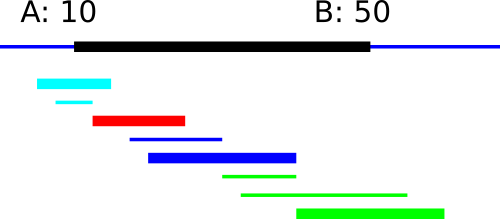
\includegraphics[width=.8\textwidth]{img/minimal_coverage_solution}\]
\end{frame}

\subsection{Bad Greedy Example}
\begin{frame}
  \frametitle{Bad Greedy Example: Coin Change}

  Given a target value $V$ and a set of coin sizes $S$, select a group $C$ of coins (with repetition) that adds to $V$, so that the size of $C$ is minimum.
  \bigskip

  {\bf Example Input:} $V = 42, S = \{25, 10, 5, 1\}$\bigskip
    %{\small (a 1\$ coin means we can always make any value)}

  {\bf Example Output:} $25 + 10 + 5 + 1 + 1$: Size 5\bigskip

  \begin{block}{Greedy Algorithm}
    \begin{itemize}
      \item Greedy Step: Add one coin to $C$
      \item "Best" Step: Add the biggest possible coin
    \end{itemize}
  \end{block}
\end{frame}

\begin{frame}{Bad Greedy Example: Coin Change}{Wrong Answer!}
  \begin{block}{Sample Data -- Greedy works here.}
    \begin{itemize}
      \item $V = 42, S = \{ 25, 10, 5, 1\}, C = \emptyset$, Take 25
      \item $V = 17, S = \{ 25, 10, 5, 1\}, C = \{25\}$, Take 10
      \item $V = 7, S = \{ 25, 10, 5, 1\}, C = \{25, 10\}$, Take 5
      \item $V = 2, S = \{ 25, 10, 5, 1\}, C = \{25, 10, 5\}$, Take 1
      \item $V = 1, S = \{ 25, 10, 5, 1\}, C = \{25, 10, 5, 1\}$, Take 1
    \end{itemize}
  \end{block}

  \begin{alertblock}{Trick Case! $\{3, 3\} < \{4, 1, 1\}$ -- There is no "best step" rule for this problem}
    \begin{itemize}
      \item $V = 6, S = \{4,3,1\}, C = \emptyset$, take 4
      \item $V = 2, S = \{4,3,1\}, C = \{4\}$, take 1
      \item $V = 1, S = \{4,3,1\}, C = \{4,1\}$, take 1
    \end{itemize}
  \end{alertblock}
\end{frame}
